\documentclass[10pt]{article}

%%%%%%%%%%%%%%%%%%%%%%%%%%%%%%%%%%%%%%%%%%%%%%%%%%%%%%%%%%%%%%%%%%%%%%%%%%%%%%%
%%% packages %%%
%%%%%%%%%%%%%%%%%%%%%%%%%%%%%%%%%%%%%%%%%%%%%%%%%%%%%%%%%%%%%%%%%%%%%%%%%%%%%%%

\usepackage[english]{babel} % Choose english language
\usepackage[labelfont = bf, font = small]{caption} % Use caption package. Use bold font for caption.
\usepackage{siunitx} % Use siunitx for unit representation.
\newcommand{\RM}[1]{\MakeUppercase{\romannumeral #1{:}}}
\usepackage{graphicx}
\usepackage{tabularx}
\usepackage{float}
\usepackage{lmodern}
\usepackage{filecontents}
\usepackage{amsmath}
\usepackage{amssymb}
\usepackage[utf8]{inputenc}
\usepackage[bottom]{footmisc}
\usepackage{leftidx}
\usepackage{subcaption}
\usepackage[explicit]{titlesec}
\usepackage{booktabs}
\usepackage{multirow}
\usepackage{multicol}
\usepackage{listings}
\usepackage{enumitem}
\usepackage{pgfplots}
\usepackage{natbib}
\usepackage{xcolor}
\usepackage{url}
\usepackage{array}
\usepackage{setspace}
\usepackage{hyperref} % Referencing
\usepackage{verbatim}
\usepackage{changepage}
\usepackage[footnote, printonlyused]{acronym}
\usepackage{scrextend}
\usepackage{geometry} % Change geometry of page layout
\usepackage{rotating}
\usepackage{longtable}
\usepackage{lscape}
\usepackage{tocloft}
\usepackage{tkz-euclide}
\usepackage{listings}
\usepackage{feynmp-auto} % Create fenynman diagrams
\usepackage{tikz-feynman} % Create fenynman diagrams
\usepackage{lipsum} % For testing. insert random text

%%%%%%%%%%%%%%%%%%%%%%%%%%%%%%%%%%%%%%%%%%%%%%%%%%%%%%%%%%%%%%%%%%%%%%%%%%%%%%%
%%% new commands and environments %%%
%%%%%%%%%%%%%%%%%%%%%%%%%%%%%%%%%%%%%%%%%%%%%%%%%%%%%%%%%%%%%%%%%%%%%%%%%%%%%%%

% Create custom font
\newenvironment{myfont}{\fontfamily{put}\selectfont}{\par}

% Adapt spacing between lines
%\doublespacing

% Delete dots from toc
\renewcommand{\cftdot}{}

% Change section label to roman
\renewcommand{\thesection}{\Roman{section}}

% Customize section layout
\newcommand{\ssection}[1]{%
  \section[#1]{\centering\normalfont\scshape #1}}
\newcommand{\ssubsection}[1]{%
  \subsection[#1]{\centering\normalfont\itshape #1}}
\newcommand{\ssubsubsection}[1]{%
  \subsubsection[#1]{\centering\normalfont #1}}

% Import tikz libraries for figures
\usetikzlibrary{positioning,shadows,arrows}

% Create footnotereferencing
\makeatletter
\newcommand\footnoteref[1]{\protected@xdef\@thefnmark{\ref{#1}}\@footnotemark}
\makeatother

% Change layout of page
\hypersetup{
  colorlinks = true,
  linkbordercolor = {red},
  citebordercolor = {red},
  menubordercolor = {blue},
  urlbordercolor = {blue},
  linktoc = {page},
  pagebackref = {True},
  pdftitle = {Solution 11},
  pdfauthor = {Nils Hoyer, Maurice Morgenthaler},
  pdfcreator  = {pdflatex},
  pdfproducer = {LaTeX}
}

% Change geometry of page
\geometry{a4paper, top = 20mm, left = 20mm, right = 20mm, bottom = 15mm, headsep = 8mm, footskip = 10mm, includeheadfoot}

% Decalre uits for SIunitx
\DeclareSIUnit\femtobarn{fb^{-1}}
\DeclareSIUnit\percent{\%}

% Define colors
\definecolor{deepblue}{rgb}{0,0,0.5}
\definecolor{deepred}{rgb}{0.6,0,0}
\definecolor{deepgreen}{rgb}{0,0.6,0.2}
\definecolor{deeporange}{rgb}{0.9,0.2,0}

% Commands for further use
\newcommand{\testStat}{\tilde{q}_{\mu}}
\newcommand{\lL}[2]{\mathcal{L}\left(#1 \middle|#2 \right)}
\newcommand{\likelihood}{\mathfrak{L}}
%%%%%%%%%%%%%%%%%%%%%%%%%%%%%%%%%%%%%%%%%%%%%%%%%%%%%%%%%%%%%%%%%%%%%%%%%%%%%%%
%%% start document %%%
%%%%%%%%%%%%%%%%%%%%%%%%%%%%%%%%%%%%%%%%%%%%%%%%%%%%%%%%%%%%%%%%%%%%%%%%%%%%%%%

\begin{document}
\begin{myfont}
\lstset{language=C++,
  basicstyle=\ttfamily,
  keywordstyle=\color{blue}\ttfamily,
  stringstyle=\color{red}\ttfamily,
  commentstyle=\color{green}\ttfamily,
  morecomment=[l][\color{magenta}]{\#}
}

\begin{center}
  \begin{Large}
    \textsc{Solution for homework assignment no. 12} \\
  \end{Large}
  \vspace*{0.4cm}
    Nils Hoyer, Maurice Morgenthaler
  \vspace*{1cm}
\end{center}

\section*{Exercise 12.1}
In this exercise we had to calculate the upper limit of the $\Omega$-baryon lifetime.

Our given starting points were:

\begin{itemize}
    \item Estimator: observed decay time $\tau_0 = \si{0.7 \cdot 10^{-10}s}$
    \item Reference sample: 
    
    observations of an exponential decay:
        \begin{equation}
            f_{\tau}(\tau_0) = p(\tau_0|\tau) = \frac{1}{\tau} \exp{\left(-\frac{\tau_0}{\tau}\right)}
        \end{equation}
    Cumulative version:
        \begin{equation}
            F_{\tau}(\tau) = 1 - \exp{\left(-\frac{\tau_0}{\tau}\right)}
        \end{equation}
    \item Ordering rule: upper limit $F_{\tau_{up}}=\alpha$
    \item Confidence level: $1 - \alpha = 0.68$
\end{itemize}

Step 1: The acceptance region is defined for a chosen $\tau$ by all $\tau_0$ full filling the condition:
    \begin{equation}
        F_{\tau}(\tau_0) = 1 - \exp{\left(-\frac{\tau_0}{\tau}\right)} \geq \alpha
        => \tau_0 \geq -\tau \log(1-\alpha)
    \end{equation}
    
\begin{figure}
    \centering
    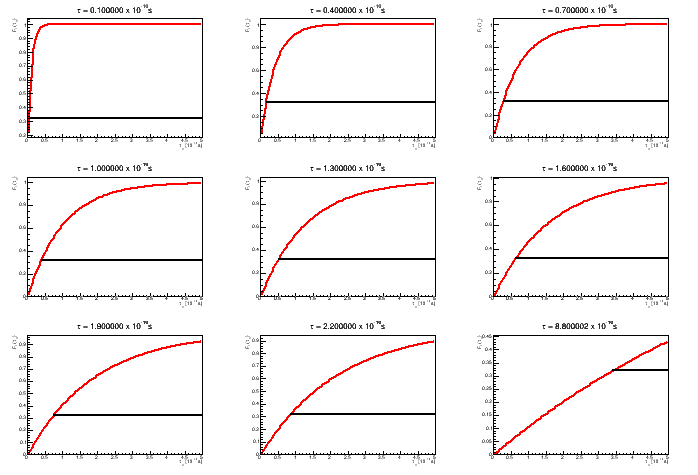
\includegraphics[width=0.9\textwidth]{exercise12_1a.png}
    \caption{Visualization of the acceptance region for some $\tau$. The red line is the cumulative exponential function while the black line represents the acceptance region}
    \label{fig:accRegion}
\end{figure}

Plotting the acceptance regions of figure \ref{fig:accRegion} into figure \ref{fig:upperCI} with $\tau$ plotted against $\tau_0$ results in a red confident belt. The intersection between the blue estimator of $tau_0$ gives us the upper limit of $\tau$ (green). Therefore the confidence interval is given by $\tau \leq 1.815 \cdot 10^{-10} \si{s}$.  

\begin{figure}
    \centering
    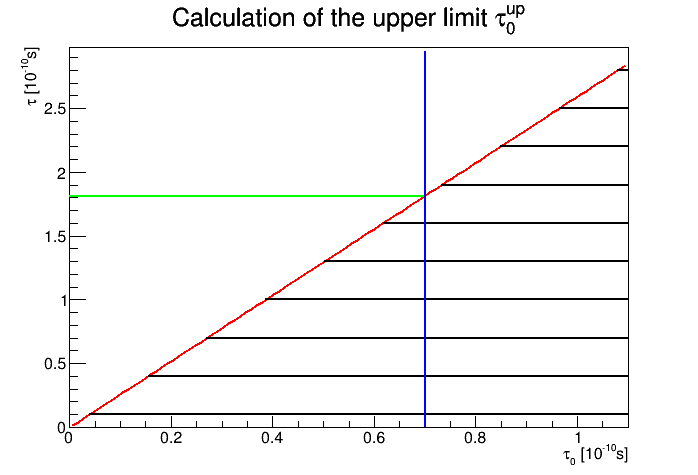
\includegraphics[width=0.9\textwidth]{exercise12_1b.png}
    \caption{Visualization of confidence interval. The red line shows the confidence belt created from the black acceptance regions. The blue line is the estimator while the green one gives us the value of the upper limit.}
    \label{fig:upperCI}
\end{figure}

\section*{Exercise 12.2}

\end{myfont}
\end{document}\documentclass{article}
